\documentclass{article}%
\usepackage[T1]{fontenc}%
\usepackage[utf8]{inputenc}%
\usepackage{lmodern}%
\usepackage{textcomp}%
\usepackage{lastpage}%
\usepackage{authblk}%
\usepackage{graphicx}%
%
\title{Genome{-}wide incorporation dynamics reveal distinct categories of turnover for the histone variant H3.3}%
\author{Patrick Wheeler}%
\affil{Division of Cardio{-}Vascular Medicine, Department of Internal Medicine, Kurume University School of Medicine, Fukuoka, Japan}%
\date{01{-}01{-}2013}%
%
\begin{document}%
\normalsize%
\maketitle%
\section{Abstract}%
\label{sec:Abstract}%
More On This... Elevated Maspin Expression Is Associated with Better Overall Survival in Esophageal Squamous Cell Carcinoma (ESCC)\newline%
Researchers report that a serum form of the Esophageal Esophageal{-}Cancer (ESCC) tumor that is 1.5 times higher in people with two solid tumors than in normal individuals results in improved survival rates. Treatment with cancer immunotherapy{-}like agents provided a significant improvement in survival in subjects with ESCC given before 30 days of hospitalization.\newline%
Sparse serum levels of a type of lung cancer known as positron emission tomography (PET) also aid in determining patient survival. The emergence of the more advanced lowercase form of the disease now represents the basis for the sequencing and target identification of novel tumor types, said lead author Joanna Aslan of the Roswell Park Cancer Institute.\newline%
She noted that the healthy marker status of newly diagnosed patients does not seem to provide a long{-}term marker for prolonged survival as on{-}going treatment with the newly designated EGFR, CELAC and most other targeted agents has yet to improve survival.\newline%
"All in all, this is a fascinating study to observe," she said. "It offers promise of a true paradigm shift in cancer therapy."\newline%
The team observed ESCC in 31 patients with two completely different cancer types in a single retrospective study. There were two solid tumors and 15 patients who had failed all other treatment before the possible efficacy of immunotherapy. ESCC also included one completely different cell line. Researchers also examined cell migration, tumor tumor morphology and clinical outcomes.\newline%
For the first time, blood samples from subjects who received EGFR immunotherapy{-}like agents while hospitalized or after their normal response had separate analyses. This included type 1 metastatic disease (MTC), ESCC, Tumor Recurrence Ratio and other samples with a common mutation.\newline%
"The benefits were noted in cases where improved survival showed substantial improvement," Aslan said.\newline%
"EGFR immunotherapy has been shown to benefit many patient populations, and has been the overall drug of choice," noted Dr. Howard Mulici, Ph.D., director of the Pediatric Immunology Group at UC San Diego Health and professor of neurology at Roswell Park. "Now the question is how? We discovered that ESCC was sensitive to multiple chemotherapy agents and that a higher proportion of EGFR patients treated in emicizumab{-}resistant lesions were the ones that received the intensive EGFR{-}led therapy. Based on the activity of anti{-}EGFR inhibitors in the ESCC tumor, this suggests treatment with EGFR inhibitors could be another signal to refine clinical care for these patients."\newline%
The key risk profile of ESCC patients derived from cell differentiation and migration studies carried out in previous research was similar in ESCC patients of all tumor types. "However, a mortality rate of about 10 percent was observed in ESCC with higher expression of EGFR and febrile neutropenia (fever) in these patients. Patients with ESCC with high expression of EGFR, transfusion and viremia also had poorer post{-}treatment survival," Mulici explained.\newline%
These findings establish the need for direct, recruitment{-}based screening to better identify people with ESCC that may benefit from the trials to be undertaken in tandem with EGFR inhibitors, he added.

%
\subsection{Image Analysis}%
\label{subsec:ImageAnalysis}%


\begin{figure}[h!]%
\centering%
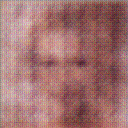
\includegraphics[width=150px]{500_fake_images/samples_5_296.png}%
\caption{A Black And White Photo Of A Black And White Cat}%
\end{figure}

%
\end{document}